\documentclass[12pt,a4paper,fleqn,leqno]{article}
\usepackage{mathtext}
\usepackage{cmap}
\usepackage[utf8x]{inputenc}
\usepackage[russian]{babel}
\usepackage[T2A]{fontenc}
\usepackage{amsmath,amssymb,amsthm,amscd,amsfonts}
\usepackage{euscript}
\usepackage{relsize}
\usepackage{mathdots}
\usepackage{graphicx}
\usepackage{epstopdf}
\usepackage{caption2}
\usepackage{indentfirst}
\usepackage{fancyhdr}
\usepackage{sectsty}
\usepackage{titlesec}
\usepackage{sicpro_rus}
\usepackage{mathtext}%русские буквы в формулах

\usepackage[colorlinks, urlcolor=blue, pdfborder={0 0 0 [0 0]}]{hyperref}

\hyphenation{Struc-tu-red}
\hyphenation{Ran-do-mized}
\hyphenation{Ma-xi-mi-za-tion}
\DeclareMathOperator*{\argmax}{arg\,max}
\DeclareMathOperator*{\argmin}{arg\,min}
\DeclareMathOperator{\tr}{tr}
\providecommand*{\BibDash}{}

\def\rank{\mathop{\mathrm{rank}}}
\newtheorem{corollary}{Следствие}
\newtheorem{proposition}{Предложение}
\newtheorem{algorithm}{Алгоритм}
\newtheorem{lemma}{Лемма}

%new calligraphic font for subspaces
\usepackage{euscript}
\newcommand{\spA}{\EuScript{A}}
\newcommand{\spB}{\EuScript{B}}
\newcommand{\spC}{\EuScript{C}}
\newcommand{\spD}{\EuScript{D}}
\newcommand{\spE}{\EuScript{E}}
\newcommand{\spF}{\EuScript{F}}
\newcommand{\spG}{\EuScript{G}}
\newcommand{\spH}{\EuScript{H}}
\newcommand{\spI}{\EuScript{I}}
\newcommand{\spJ}{\EuScript{J}}
\newcommand{\spK}{\EuScript{K}}
\newcommand{\spL}{\EuScript{L}}
\newcommand{\spM}{\EuScript{M}}
\newcommand{\spN}{\EuScript{N}}
\newcommand{\spO}{\EuScript{O}}
\newcommand{\spP}{\EuScript{P}}
\newcommand{\spQ}{\EuScript{Q}}
\newcommand{\spR}{\EuScript{R}}
\newcommand{\spS}{\EuScript{S}}
\newcommand{\spT}{\EuScript{T}}
\newcommand{\spU}{\EuScript{U}}
\newcommand{\spV}{\EuScript{V}}
\newcommand{\spW}{\EuScript{W}}
\newcommand{\spX}{\EuScript{X}}
\newcommand{\spY}{\EuScript{Y}}
\newcommand{\spZ}{\EuScript{Z}}

%font for text indices like transposition X^\mathrm{T}
\newcommand{\rmA}{\mathrm{A}}
\newcommand{\rmB}{\mathrm{B}}
\newcommand{\rmC}{\mathrm{C}}
\newcommand{\rmD}{\mathrm{D}}
\newcommand{\rmE}{\mathrm{E}}
\newcommand{\rmF}{\mathrm{F}}
\newcommand{\rmG}{\mathrm{G}}
\newcommand{\rmH}{\mathrm{H}}
\newcommand{\rmI}{\mathrm{I}}
\newcommand{\rmJ}{\mathrm{J}}
\newcommand{\rmK}{\mathrm{K}}
\newcommand{\rmL}{\mathrm{L}}
\newcommand{\rmM}{\mathrm{M}}
\newcommand{\rmN}{\mathrm{N}}
\newcommand{\rmO}{\mathrm{O}}
\newcommand{\rmP}{\mathrm{P}}
\newcommand{\rmQ}{\mathrm{Q}}
\newcommand{\rmR}{\mathrm{R}}
\newcommand{\rmS}{\mathrm{S}}
\newcommand{\rmT}{\mathrm{T}}
\newcommand{\rmU}{\mathrm{U}}
\newcommand{\rmV}{\mathrm{V}}
\newcommand{\rmW}{\mathrm{W}}
\newcommand{\rmX}{\mathrm{X}}
\newcommand{\rmY}{\mathrm{Y}}
\newcommand{\rmZ}{\mathrm{Z}}

%tt font for time series
\newcommand{\tsA}{\mathbb{A}}
\newcommand{\tsB}{\mathbb{B}}
\newcommand{\tsC}{\mathbb{C}}
\newcommand{\tsD}{\mathbb{D}}
\newcommand{\tsE}{\mathbb{E}}
\newcommand{\tsF}{\mathbb{F}}
\newcommand{\tsG}{\mathbb{G}}
\newcommand{\tsH}{\mathbb{H}}
\newcommand{\tsI}{\mathbb{I}}
\newcommand{\tsJ}{\mathbb{J}}
\newcommand{\tsK}{\mathbb{K}}
\newcommand{\tsL}{\mathbb{L}}
\newcommand{\tsM}{\mathbb{M}}
\newcommand{\tsN}{\mathbb{N}}
\newcommand{\tsO}{\mathbb{O}}
\newcommand{\tsP}{\mathbb{P}}
\newcommand{\tsQ}{\mathbb{Q}}
\newcommand{\tsR}{\mathbb{R}}
\newcommand{\tsS}{\mathbb{S}}
\newcommand{\tsT}{\mathbb{T}}
\newcommand{\tsU}{\mathbb{U}}
\newcommand{\tsV}{\mathbb{V}}
\newcommand{\tsW}{\mathbb{W}}
\newcommand{\tsX}{\mathbb{X}}
\newcommand{\tsY}{\mathbb{Y}}
\newcommand{\tsZ}{\mathbb{Z}}

%bf font for matrices
\newcommand{\bfA}{\mathbf{A}}
\newcommand{\bfB}{\mathbf{B}}
\newcommand{\bfC}{\mathbf{C}}
\newcommand{\bfD}{\mathbf{D}}
\newcommand{\bfE}{\mathbf{E}}
\newcommand{\bfF}{\mathbf{F}}
\newcommand{\bfG}{\mathbf{G}}
\newcommand{\bfH}{\mathbf{H}}
\newcommand{\bfI}{\mathbf{I}}
\newcommand{\bfJ}{\mathbf{J}}
\newcommand{\bfK}{\mathbf{K}}
\newcommand{\bfL}{\mathbf{L}}
\newcommand{\bfM}{\mathbf{M}}
\newcommand{\bfN}{\mathbf{N}}
\newcommand{\bfO}{\mathbf{O}}
\newcommand{\bfP}{\mathbf{P}}
\newcommand{\bfQ}{\mathbf{Q}}
\newcommand{\bfR}{\mathbf{R}}
\newcommand{\bfS}{\mathbf{S}}
\newcommand{\bfT}{\mathbf{T}}
\newcommand{\bfU}{\mathbf{U}}
\newcommand{\bfV}{\mathbf{V}}
\newcommand{\bfW}{\mathbf{W}}
\newcommand{\bfX}{\mathbf{X}}
\newcommand{\bfY}{\mathbf{Y}}
\newcommand{\bfZ}{\mathbf{Z}}

%bb font for standard spaces and expectation
\newcommand{\bbA}{\mathbb{A}}
\newcommand{\bbB}{\mathbb{B}}
\newcommand{\bbC}{\mathbb{C}}
\newcommand{\bbD}{\mathbb{D}}
\newcommand{\bbE}{\mathbb{E}}
\newcommand{\bbF}{\mathbb{F}}
\newcommand{\bbG}{\mathbb{G}}
\newcommand{\bbH}{\mathbb{H}}
\newcommand{\bbI}{\mathbb{I}}
\newcommand{\bbJ}{\mathbb{J}}
\newcommand{\bbK}{\mathbb{K}}
\newcommand{\bbL}{\mathbb{L}}
\newcommand{\bbM}{\mathbb{M}}
\newcommand{\bbN}{\mathbb{N}}
\newcommand{\bbO}{\mathbb{O}}
\newcommand{\bbP}{\mathbb{P}}
\newcommand{\bbQ}{\mathbb{Q}}
\newcommand{\bbR}{\mathbb{R}}
\newcommand{\bbS}{\mathbb{S}}
\newcommand{\bbT}{\mathbb{T}}
\newcommand{\bbU}{\mathbb{U}}
\newcommand{\bbV}{\mathbb{V}}
\newcommand{\bbW}{\mathbb{W}}
\newcommand{\bbX}{\mathbb{X}}
\newcommand{\bbY}{\mathbb{Y}}
\newcommand{\bbZ}{\mathbb{Z}}

%got font for any case
\newcommand{\gA}{\mathfrak{A}}
\newcommand{\gB}{\mathfrak{B}}
\newcommand{\gC}{\mathfrak{C}}
\newcommand{\gD}{\mathfrak{D}}
\newcommand{\gE}{\mathfrak{E}}
\newcommand{\gF}{\mathfrak{F}}
\newcommand{\gG}{\mathfrak{G}}
\newcommand{\gH}{\mathfrak{H}}
\newcommand{\gI}{\mathfrak{I}}
\newcommand{\gJ}{\mathfrak{J}}
\newcommand{\gK}{\mathfrak{K}}
\newcommand{\gL}{\mathfrak{L}}
\newcommand{\gM}{\mathfrak{M}}
\newcommand{\gN}{\mathfrak{N}}
\newcommand{\gO}{\mathfrak{O}}
\newcommand{\gP}{\mathfrak{P}}
\newcommand{\gQ}{\mathfrak{Q}}
\newcommand{\gR}{\mathfrak{R}}
\newcommand{\gS}{\mathfrak{S}}
\newcommand{\gT}{\mathfrak{T}}
\newcommand{\gU}{\mathfrak{U}}
\newcommand{\gV}{\mathfrak{V}}
\newcommand{\gW}{\mathfrak{W}}
\newcommand{\gX}{\mathfrak{X}}
\newcommand{\gY}{\mathfrak{Y}}
\newcommand{\gZ}{\mathfrak{Z}}

%old calligraphic font
\newcommand{\calA}{\mathcal{A}}
\newcommand{\calB}{\mathcal{B}}
\newcommand{\calC}{\mathcal{C}}
\newcommand{\calD}{\mathcal{D}}
\newcommand{\calE}{\mathcal{E}}
\newcommand{\calF}{\mathcal{F}}
\newcommand{\calG}{\mathcal{G}}
\newcommand{\calH}{\mathcal{H}}
\newcommand{\calI}{\mathcal{I}}
\newcommand{\calJ}{\mathcal{J}}
\newcommand{\calK}{\mathcal{K}}
\newcommand{\calL}{\mathcal{L}}
\newcommand{\calM}{\mathcal{M}}
\newcommand{\calN}{\mathcal{N}}
\newcommand{\calO}{\mathcal{O}}
\newcommand{\calP}{\mathcal{P}}
\newcommand{\calQ}{\mathcal{Q}}
\newcommand{\calR}{\mathcal{R}}
\newcommand{\calS}{\mathcal{S}}
\newcommand{\calT}{\mathcal{T}}
\newcommand{\calU}{\mathcal{U}}
\newcommand{\calV}{\mathcal{V}}
\newcommand{\calW}{\mathcal{W}}
\newcommand{\calX}{\mathcal{X}}
\newcommand{\calY}{\mathcal{Y}}
\newcommand{\calZ}{\mathcal{Z}}

%sf font for transposition and spaces like R
\newcommand{\sfA}{\mathsf{A}}
\newcommand{\sfB}{\mathsf{B}}
\newcommand{\sfC}{\mathsf{C}}
\newcommand{\sfD}{\mathsf{D}}
\newcommand{\sfE}{\mathsf{E}}
\newcommand{\sfF}{\mathsf{F}}
\newcommand{\sfG}{\mathsf{G}}
\newcommand{\sfH}{\mathsf{H}}
\newcommand{\sfI}{\mathsf{I}}
\newcommand{\sfJ}{\mathsf{J}}
\newcommand{\sfK}{\mathsf{K}}
\newcommand{\sfL}{\mathsf{L}}
\newcommand{\sfM}{\mathsf{M}}
\newcommand{\sfN}{\mathsf{N}}
\newcommand{\sfO}{\mathsf{O}}
\newcommand{\sfP}{\mathsf{P}}
\newcommand{\sfQ}{\mathsf{Q}}
\newcommand{\sfR}{\mathsf{R}}
\newcommand{\sfS}{\mathsf{S}}
\newcommand{\sfT}{\mathsf{T}}
\newcommand{\sfU}{\mathsf{U}}
\newcommand{\sfV}{\mathsf{V}}
\newcommand{\sfW}{\mathsf{W}}
\newcommand{\sfX}{\mathsf{X}}
\newcommand{\sfY}{\mathsf{Y}}
\newcommand{\sfZ}{\mathsf{Z}}

\newcommand{\bt}{\begin{theorem}}
\newcommand{\et}{\end{theorem}}
\newcommand{\bl}{\begin{lemma}}
\newcommand{\el}{\end{lemma}}
\newcommand{\bp}{\begin{proposition}}
\newcommand{\ep}{\end{proposition}}
\newcommand{\bc}{\begin{corollary}}
\newcommand{\ec}{\end{corollary}}

\newcommand{\bd}{\begin{definition}\rm}
\newcommand{\ed}{\end{definition}}
\newcommand{\bex}{\begin{example}\rm}
\newcommand{\eex}{\end{example}}
\newcommand{\br}{\begin{remark}\rm}
\newcommand{\er}{\end{remark}}

\newcommand{\btbh}{\begin{table}[!ht]}
\newcommand{\etb}{\end{table}}
\newcommand{\bfgh}{\begin{figure}[!ht]}
\newcommand{\efg}{\end{figure}}

\newcommand{\bea}{\begin{eqnarray*}}
\newcommand{\eea}{\end{eqnarray*}}
\newcommand{\be}{\begin{eqnarray}}
\newcommand{\ee}{\end{eqnarray}}
%
\newcommand{\intl}{\int\limits}
\newcommand{\suml}{\sum\limits}
\newcommand{\liml}{\lim\limits}
\newcommand{\prodl}{\prod\limits}
\newcommand{\minl}{\min\limits}
\newcommand{\maxl}{\max\limits}
\newcommand{\supl}{\sup\limits}
%
\newcommand{\ve}{\varepsilon}
\newcommand{\vphi}{\varphi}
\newcommand{\ovl}{\overline}
\newcommand{\lm}{\lambda}
\def\wtilde{\widetilde}
\def\what{\widehat}

\newcommand{\ra}{\rightarrow}
\newcommand{\towith}[1]{\mathrel{\mathop{\longrightarrow}_{#1}}}

\def\bproof{\textbf{Proof.\ }}
\def\eproof{\hfill$\Box$\smallskip}

\def\spaceN{\mathsf{N}}
\def\spaceZ{\mathsf{Z}}
\def\spaceR{\mathsf{R}}
\def\spaceC{\mathsf{C}} %is not used?
\newcommand\Expect{\mathsf{E}}
%\newcommand\Variance{\mathsf{D}}

\newcommand{\bfw}{\mathbf{w}}

\def\last#1{{\underline{#1}}}
\def\llast#1{\underline{\underline{#1}}}
\def\first#1{{\mathstrut\overline{#1}}}
\def\ffirst#1{\mathstrut\overline{\mathstrut\overline{#1}}}
\def\overo#1{\overset{_\mathrm{o}}{#1}}
\newcommand{\ontop}[2]{\genfrac{}{}{0pt}{0}{#1}{#2}}
\def\bfpi{\mbox{\boldmath{$\pi$}}}
\def\bfmu{\mbox{\boldmath{$\mu$}}}
\def\bfPi{\mbox{\boldmath{$\Pi$}}}
\def\bfcR{\mbox{\boldmath{$\cR$}}}

\def\mmod{\mathop{\mathrm{mod}}}
\def\sspan{\mathop{\mathrm{span}}}
\def\rank{\mathop{\mathrm{rank}}}
\def\dist{\mathop{\mathrm{dist}}}

\newcommand{\reverse}{\mathop{\mathrm{rev}}}
\newcommand{\Arg}{\mathop\mathrm{Arg}}
\newcommand{\meas}{\mathop{\mathrm{meas}}}

\newcommand{\colspace}{\mathop{\mathrm{colspace}}}
\newcommand{\rowspace}{\mathop{\mathrm{rowspace}}}


\makeatletter
\def\adots{\mathinner{\mkern2mu\raise\p@\hbox{.}
\mkern2mu\raise4\p@\hbox{.}\mkern1mu
\raise7\p@\vbox{\kern7\p@\hbox{.}}\mkern1mu}}
\newcommand{\l@abcd}[2]{\hbox to\textwidth{#1\dotfill #2}}
\makeatother

\def\func{\mathop\mathrm}

% Some new definitions
\newcommand{\defeq}{\stackrel{def}{=}}
\newcommand{\frob}{\calF}
\def\trajmat#1{\calT_{\mathrm{#1}}}

\def\unit{\mathfrak{i}}



\sectionfont{\centering}

\subsectionfont{\centering}
\subsubsectionfont{\normalsize}
\setcounter{page}{1}


\author{Nikita Zvonarev}
\title{Iterative algorithms for Weighted Finite Rank Time Series  Approximation}
\begin{document}
\noindent УДК 519.246.8+519.254

\begin{center}{
\fontsize{18pt}{23pt}\selectfont\bf%
  \MakeUppercase{
 Iterative algorithms for Weighted Finite Rank Time Series Approximation
}}
\end{center}

\begin{center}{\bpv\bmv {Nikita Zvonarev}\\
\footnotesize\it St.Petersburg State University,\\
Department of Statistical Modelling
\\
\rm
E-mail: \textcolor {blue}{\underline{nikitazvonarev@gmail.com}}}
\end{center}
\begin{center}{\bpv {Nina Golyandina}\\
\footnotesize\it St.Petersburg State University,\\
Department of Statistical Modelling
\\
\rm
E-mail: \textcolor {blue}{\underline{nina@gistatgroup.com}}}
\end{center}
\hspace{1.25cm}\begin{minipage}{12.16cm}\bpv\bpv\bmv \noindent
\footnotesize{\bf Keywords:}\/ time series, Cadzow iterations, time series of finite rank, weighted total least squares, oblique SVD-factorization, singular spectrum analysis

\bpv\bpv\noindent  The problem of time series approximation by series of finite rank is considered in the paper. This is actual problem in signal processing tasks, partially, for extracting a signal in analysis of noisy signals. After applying weigthed least-squares method, the optimization problem arises, which do not have an exact solution. One of the numeric local minimum search method (Cadzow iterations) is well known. However, Cadzow iterations may work with specific weights only, which decreases while approaching edges of time series. In addition, it is naturally to take equal weights corresponding to usual Euclidean metric. Therefore, several new methods are suggested and investigated to achieve equal or approximately equal weights. Questions of convergency, computational complexity and accuracy are considered for proposed methods. Methods are compared on the numeric example.\footnote{Переписать}

\end{minipage}\bls\bmv

\section{Introduction}
Consider the problem of extracting a signal $\tsS = (s_1, \ldots, s_N)$ from an observed noisy signal $\tsX = \tsS + \tsN$, where $\tsS$ is governed by a \emph{linear recurrence relation} (LRR) of order $r$:
\begin{equation*}
s_n = \sum_{i = 1}^{r} a_i s_{n-i}, \quad n = r + 1, \ldots, N.
\end{equation*}
Generally, governed-by-LRR series may be written in a parametric form 
\begin{equation} \label{parametricform}
s_n = \sum_i P_i(n) \exp(\alpha_i n) \cos(2 \pi \omega_i n + \psi_i)
\end{equation}, where $P_i(n)$ in \eqref{parametricform} are polynomials. However, parametric regression approach for the problem does not lead to accurate estimation of parameters due to their large amount and instability of estimators.

It is known that methods based on signal subspace estimation (subspace-based methods) works well. \footnote{ссылки} These subspace-based methods use the following approach: let us fix window length $L$, $1 \le L \le N$, $K = N - L + 1$, and build the trajectory matrix for the series $\tsS$:
\begin{equation*}
\bfS = \begin{pmatrix}
s_1 & s_2 & \ldots & s_K \\
s_2 & s_3 & \ldots & s_{K + 1} \\
\vdots & \vdots & \vdots & \vdots \\
s_L & s_{L + 1} & \ldots & s_N
\end{pmatrix}.
\end{equation*}
Note that $\bfS\in \calH$, where $\calH$ is the set of Hankel matrices with equal values on their anti-diagonals $i+j=\mathrm{const}$.
If $\tsS$ is governed by a minimal LRR of order $r$, $r < \min(L, K)$, then $\rank \bfS = r$. So, $\bfS$ is a Hankel matrix of low-rank $r$. Column space of $\bfS$ provides estimates of $\alpha_i$ and $\omega_i$ in \eqref{parametricform} by the ESPRIT method.

Let $\bfX$ be the trajectory matrix of the series $\tsX$. Then the problem of estimation of $\tsS$ can be considered as the problem of approximation of matrix $\bfX$ by a Hankel matrix of rank not larger than $r$:
\begin{equation}\label{introd_task}
\|\bfX - \bfY\|^2_\rmF \to \min_{\substack{\rank \bfY \le r \\ \bfY \in \calH}}.
\end{equation}

A lot of papers are dedicated to this problem, e.g., \cite{Cadzow1988, Markovsky2011, Usevich.Markovsky2014, Gillard.Zhigljavsky2013} among them, where the problem is called Structured Low-Rank Approximation. Approaches to solving the problem are iterative, e.g., Cadzow iterations \cite{Cadzow1988} consist of alternating projections to the set of Hankel matrices and matrices of rank not larger than $r$. The target function is not unimodal in such class of problems, and convergency to global minimum is not guaranteed; despite this, problem \eqref{introd_task} is considered to be well-researched, though it has many open answers yet.

Note that problem \eqref{introd_task} is equivalent to the problem of weighted approximation of the series $\tsX = (x_1, \ldots, x_N)$:
\begin{equation}\label{introd_task_2}
\sum_{i = 1}^N w_i(x_i - y_i)^2 \to \min_{\substack{\tsY: \rank \bfY \le r \\ \bfY \in \calH}},
\end{equation}
where
\begin{equation}
\label{eq:w}
w_i = \begin{cases}
i & \text{for $i = 1, \ldots, L-1,$}\\
L & \text{for $i = L, \ldots, K,$}\\
N - i + 1 & \text{for $i = K + 1, \ldots, N.$}
\end{cases}.
\end{equation}

Weights on edges of series are less than in the center, i.e. ordinary LS problem \eqref{introd_task} for matrices is a weighted least squares problem for series.

The aim of this paper is to consider methods which solve problem \eqref{introd_task_2} with arbitrary weights instead of $w_i$ and compare methods in terms of precision of the signal estimation. All described methods are iterative. If an estimate of the signal, which is not governed by LRR, is the point of interest then only the first iteration can be taken with aim of reduction of computational complexity. So, described methods are compared by precision of the signal estimation in the first iteration and in the limit. Note that known Singular Spectrum Analysis (SSA) \cite{Broomhead.King1986, Vautard.etal1992, Elsner.Tsonis1996, Golyandina.etal2001, Ghil.etal2002, Golyandina.Zhigljavsky2012} can be
described as one iteration of the Cadzow method.

Structure of paper is as follows.  In Section~\ref{sec:lowrank_appr}, a problem of approximating a matrix by a Hankel rank-deficient matrix is considered. Common structure of iterative alternating projection algorithms is described, techniques (?) of construction of projectors are given, the convergency theorem is proved.

In Section~\ref{sec:ts_matrices}, the relation between problems of approximation of time series and matrices is described, relationship between weights in the corresponding weighted least squares problems is also given. Section~\ref{sec:alg} is dedicated to suggested time series approximation algorithms. In Section~\ref{sec:simul} numeric comparison of algorithms on typical example is performed.

The paper is finished with short conclusions and discussion of further work in Section~\ref{sec:concl}. The result of separability of constant and sinusoidal signal by SSA with weights, which has relation with convergency for two of the described algorithms, is proved in Appendix.

\section{Approximation by rank-deficient Hankel matrices}
\label{sec:lowrank_appr}
\subsection{Common algorithm}
Consider a problem of approximation of a matrix $\bfX$ by a Hankel rank-deficient matrix with respect to some (semi)norm $\|\cdot\|$. Define by $\spaceR^{L\times K}$ the space of matrices of size $L \times K$, $\calM_r\subset \spaceR^{L\times K}$ is the set of matrices of rank not larger than $r$,
$\calH \subset \spaceR^{L\times K}$ is the set of Hankel matrices.
Note that  $\calM_r$ is not nor linear, nor convex set. However, $\calM_r$ is multiplicative, i.e.
if $\bfZ\in \calM_r$, then $a\bfZ\in \calM_r$ for any $a$.
Space $\calH$ is linear.

The problem is
\be
\label{eq:gen_task}
\|\bfX - \bfY\| \to \min_\bfY, \mbox{\ where\ } \bfY \in \calH \cap \calM_r.
\ee

For presenting the algorithm's scheme for this problem, let us introduce projectors to the subspaces with respect to norm $\|\cdot\|$, $\Pi_{\calM_r}$ is the projector to $\calM_r$,
$\Pi_{\calH}$ is the projector to $\calH$.
Note that result of projection to $\calM_r$ can not be defined uniquely, but further we suppose that in the case of ambiguity any value from all possible is chosen. The projector to $\calH$ is evidently orthogonal, while $\Pi_{\calM_r}$ is orthognonal due to the following proposition.

\begin{proposition} \label{pythaprop}
Let $\calX$ be Hilbert space, $\calM$ is a multiplicative subset, $\Pi_\calM$ is projection operator to $\calM$. Then for any $x \in \calX$ Pythagorean theorem is true: $\|x\|^2 = \|x - \Pi_\calM x\|^2 + \|\Pi_\calM x\|^2$.
\end{proposition}
\begin{proof5}{\ref{pythaprop}}
By using multiplicativity, the set $\calM$ could be represented as $\calM = \bigcup\limits_{l \in \calL}l$, where $\calL$ is the set of all lines lying in $\calM$ and passing through $0$. Then the projection can be described as follows: to begin with, we choose a line $l$ such that $\dist(x, l) \rightarrow \min\limits_{l \in \calL}$; then, $y = \Pi_\calM x$ is the orthogonal projection of $x$ to the line $l$, which is a linear subspace. Proposition is proved.
\end{proof5}

For solving problem \eqref{eq:gen_task} the iterative method of alternating projections can be used:
\be
   \bfY_{k+1}=\Pi_\calH \Pi_{\calM_r} \bfY_{k}, \mbox{\ where\ } \bfY_{0}=\bfX.
\ee

Let us prove a theorem about convergency rate of the given method.

\begin{theorem}
\label{th:converg}
\begin{enumerate}
Let the space $\calM_r$ be closed in topology gererated by norm $\|\cdot\|$. Then
\item $\|\bfY_k - \Pi_{\calM_r}\bfY_k\| \to 0$ as $k \to +\infty$, $\|\Pi_{\calM_r}\bfY_k - \bfY_{k+1}\| \to 0$ as $k \to +\infty$.
\item There exists a convergent subsequence of matrices $\bfY_{i_1}, \bfY_{i_2}, \ldots$ such that its limit $\bfY^*$ lies in $\calM_r \cap \calH$.
\end{enumerate}
\end{theorem}
\begin{proof2}{\ref{th:converg}}
Let us use inequalities \cite{Chu.etal2003}
\begin{equation}
\label{chuprop}
\|\bfY_k - \Pi_{\calM_r} \bfY_k\| \ge \|\Pi_{\calM_r} \bfY_k - \bfY_{k + 1}\| \ge \|\bfY_{k+1} - \Pi_{\calM_r} \bfY_{k + 1}\|.
\end{equation}

\begin{enumerate}
\item According to inequalities \eqref{chuprop}, \footnote{the?} sequences $\|\bfY_k - \Pi_{\calM_r} \bfY_k\|$, $k = 1, 2, \ldots$, and $\|\Pi_{\calM_r} \bfY_k - \bfY_{k + 1}\|$, $k = 1, 2, \ldots$, are non-increasing. It is obvious that they are limited below by zero. So they have equal limits $c$ according to \eqref{chuprop}.

Prove that $c = 0$. Assume contrary: there exists $d > 0$ such that $\|\bfY_k - \Pi_{\calM_r} \bfY_k\| > d$, $\|\Pi_{\calM_r} \bfY_k - \bfY_{k + 1}\| > d$ for any $k = 1, 2, \ldots$. According to Proposition ~\ref{pythaprop}, the following equalities are true:
\begin{gather*}
\|\bfY_k\|^2 = \|\Pi_{\calM_r} \bfY_k\|^2 + \|\bfY_k - \Pi_{\calM_r} \bfY_k\|^2 =\\ \|\bfY_k - \Pi_{\calM_r} \bfY_k\|^2 + \|\Pi_{\calM_r} \bfY_k - \bfY_{k + 1}\|^2 + \|\bfY_{k + 1}\|^2.
\end{gather*}
Thus, $\|\bfY_{k+1}\|^2 < \|\bfY_k\|^2 - 2d^2$. Expanding the inequality by the same way further, we obtain that $\|\bfY_{k+j}\|^2 < \|\bfY_k\|^2 - 2 j d^2$ for any $j = 1, 2, \ldots$. Choose any $k$, e.g. $k = 1$, and $j = \lceil \|\bfY_k\|^2 / (2d^2) \rceil + 1$. Then $\|\bfY_{k+j}\|^2 < 0$, what is impossible.
\item Consider the sequence $(\Pi_{\calM_r} \bfY_k)$, $k = 1, 2, \ldots$. It is bounded because $\|\Pi_{\calM_r} \bfZ\| \le \|\bfZ\|$ and $\|\Pi_{\calH} \bfZ\| \le \|\bfZ\|$ for any $\bfZ \in \sfR^{L \times K}$ (by Prop. \ref{pythaprop}). Then a convergent subsequence $(\Pi_{\calM_r} \bfY_{i_k})$ could be chosen, denote by $\bfY^*$ its limit, wherein $\|\Pi_{\calM_r} \bfY_{i_k} - \bfY_{i_k + 1}\| = \|\Pi_{\calM_r} \bfY_{i_k} - \Pi_\calH \Pi_{\calM_r} \bfY_{i_k}\| \to 0$ as $k \to + \infty$. Taking into consideration that $\|\bfZ - \Pi_\calH \bfZ\|$ is a composition of continuous mappings, we obtain that $\|\bfY^* - \Pi_\calH \bfY^*\| = 0$ since $\calM_r$ is closed set, $\bfY^* \in \calM_r \cap \calH$. Finally, $\Pi_\calH$ is continuous mapping and therefore sequence $(\Pi_\calH \Pi_{\calM_r} \bfY_{i_k})$ is convergent to $\bfY^*$. Thus, $\bfY_{i_k + 1}$ is a required subsequence.
\end{enumerate}
\end{proof2}

Below we will consider the norms generated by weighted Frobenius inner product in form
\be
\label{eq:w_inner_prod}
\langle\bfY, \bfZ\rangle_M = \sum_{l = 1}^L \sum_{k = 1}^K m_{l, k} y_{l, k} z_{l, k}.
\ee

It is well known that $\calM_r$ is closed with respect to usual Frobenius norm. It can be proved that $\calM_r$ is closed with respect to any weighted norm \eqref{eq:w_inner_prod} when $m_{l,k} > 0$ and therefore, Theorem~\ref{th:converg} is true in the case of positive weights.


\subsection{Evaluation of projectors}

Let us consider the weighted norm $\|\cdot\|_\bfM$ generated by \eqref{eq:w_inner_prod}, that is $||\bfX||^2 = \sum_{l = 1}^L \sum_{k = 1}^K m_{l, k} x^2_{l, k}$.

\paragraph{Projector $\Pi_\calH$.} It is easy to show that $\Pi_\calH$
could be evaluated explicitly using the following proposition.

\begin{proposition}
For $\widehat{\bfY}=\Pi_\calH \bfY$
\begin{equation*}
\hat{y}_{ij} = \frac{\sum_{l,k: l+k=i+j} m_{l,k} y_{l,k}}{\sum_{l,k: l+k=i+j} m_{l,k}}.
\end{equation*}
\end{proposition}

It is impossible to derive explicit form of $\Pi_{\calM_r}$ in general case.
Consider one specific case and suggest an iterative approach to the general case.

\paragraph{Case of explicit form of projector $\Pi_{\calM_r}$.} 
Let all weights $m_{ij}=1$. Denote $\Pi_r=\Pi_{\calM_r}$ in this special case.
It is well-known that the projector $\Pi_{r} \bfY$ can be evaluated as a sum of leading components of Singular Value Decomposition of the matrix $\bfY$: let $\bfY = \bfU \mathbf{\Sigma} \bfV^\rmT$ where $\bfU$ is an orthogonal matrix of size $L \times L$, $\mathbf{\Sigma}$ is a quasi-diagonal matrix of size $L \times K$ with non-negative diagonal elements in non-increasing order, $\bfV$ is an orthogonal matrix of size $K \times K$. More definitely, denote by $L\le K$, $\Sigma = (\sigma_1, \ldots, \sigma_L)$ the vector consisting of diagonal elements of matrix $\mathbf{\Sigma}$. Denote by $\mathbf{\Sigma}_r = (\sigma^r_{l k})$ the following matrix:
\begin{equation*}
\sigma^r_{i j} = \begin{cases}
\sigma_i & \text{if $i = j, i \le r,$}\\
0 & \text{otherwise}.
\end{cases}
\end{equation*}
Then the projection could be evaluated as follows: $\Pi_{r} \bfY  = \bfU \mathbf{\Sigma}_r \bfV^\rmT$.
Next proposition describes the case when evaluation of the projector is reduced to applying the projector  $\Pi_r$.

\begin{proposition}
\label{prop:projS}
Let $\bfC$ be a symmetric semidefinite matrix of size $K \times K$ such that $\|\bfY\|_\bfM = \tr(\bfY \bfC \bfY^\rmT)$.
Suppose that the column space of a matrix $\bfY$ lies in the column space of the matrix $\bfC$.
Then
\be
\label{eq:PiMr}
\Pi_{\calM_r} \bfY = (\Pi_r \bfB) (\bfO_\bfC^{\rmT})^\dagger,
\ee
where $\bfO_\bfC$ is a matrix such that $\bfC = \bfO_\bfC^{\rmT}\bfO_\bfC$,
$\bfB = \bfY \bfO_\bfC^{\rmT}$, $(\bfO_\bfC^{\rmT})^\dagger$ denotes  Moore-Penrose pseudoinverse to the matrix $\bfO_\bfC^{\rmT}$.
\end{proposition}
\begin{proof5}{\ref{prop:projS}}
The proof is a direct consequence of the fact that еру considered norm is generated by oblique inner product in row space of a matrix $\bfY$, see details in \cite{Golyandina2013}.
\end{proof5}

\begin{remark}
Note that the conditions of Proposition~\ref{prop:projS} can be fulfilled only if $\bfC$ is diagonal.
\end{remark}

\paragraph{Projector $\Pi_{\calM_r}$ in general case.}
Since the projector can not be found explicitly, iterative algorithms are used in the general case.
One of these algorithms is described in \cite{Srebro2003}. Denote by $\odot$ the element-wise matrix product.

\begin{algorithm}
\label{alg:weightedSVD}
\textbf{Input}: initial matrix $\bfY$, rank $r$, weight matrix $\bfM$,
stop criterion STOP.

\textbf{Result}:
Matrix $\widehat\bfY$ as an estimate of $\Pi_{\calM_r} \bfY$.

\begin{enumerate}
\item
$\bfY_0 = \bfY$, $k=0$.
\item
$\bfY_{k+1} = \Pi_r(\bfY \odot \bfM + \bfY_{k} \odot (\bfU -  \bfM))$, where
$\bfU \in \sfR^{L \times K}$,  $\bfU = \begin{pmatrix}
1 & \cdots & 1 \\
\vdots & \ddots & \vdots \\
1 & \cdots & 1
\end{pmatrix}$, $k\leftarrow k+1$.
\item
If STOP then $\widehat\bfY = \bfY_k$.
\end{enumerate}
\end{algorithm}

Note that in the case, when $m_{ij}$ are equal to 0 or 1, this algorithm is an EM-algorithm \cite{Srebro2003};
hence properties of EM-algorithms are carried out and the sequence $\bfY_k$ converges to local minimum. Formally, it does not matter what values are in $\bfY$ at positions of zeros. However, these values can influence to algorithm's convergency rate.

\section{Time series and problem of matrix approximation}
\label{sec:ts_matrices}
\subsection{Problem statement for time series}
Consider a time series $\tsX = (x_1, \ldots, x_N)$ of length $N \ge 3$. Let us fix a window length $L$, $1 < L < N$, denote $K = N - L + 1$. Also consider a sequence of vectors:
\begin{equation}\label{l_lagged}
X_i = (x_i, \ldots, x_{i + L - 1})^\rmT, \qquad i = 1, \ldots, K.
\end{equation}
Define by $L$-trajectory matrix of series $\tsX$ the matrix $\bfX = [X_1:\ldots:X_K]$.

\begin{definition}
Suppose that $0 \le r \le L$. We say that a series $\tsX$ \emph{has $L$-rank $r$} if its $L$-trajectory matrix $\bfX$ has rank $r$.
\end{definition}

Note that the series $\tsX$ can have $L$-rank $r$ only when
\begin{equation}
r \le \min(L, N-L+1). \label{min_condition}
\end{equation}
We say that the window length $L$ is \emph{admittable} for fixed $r$ if it satisfies condition \eqref{min_condition}.

Further we suppose that $L$ is not larger than $K$, since the problems of approximation of $\bfX$ and of $\bfX^\rmT$ coincide.

Let $\sfX_N$ be the set of all time series of length $N$, $\sfX_N^r$ be the set of all time series of length $N$ of $L$-rank not larger than $r$. For a given time series $\tsX \in \sfX_N$, a window length $L$, $1 < L < N$, and $r$ satisfying condition \eqref{min_condition}, consider the problem:
\begin{equation} \label{L-rank_task}
f_q(\tsY) \to \min_{\tsY \in \sfX_N^r}, \quad f_q(\tsY) = \sum \limits_{i=1}^N q_i(x_i - y_i)^2,
\end{equation}
where $\tsY = (y_1, \ldots, y_N)$ and $q_1, \ldots, q_N$ are some non-negative weights,
$q_i \ge 0$, $i = 1, \ldots, N$. The one of the most interest target function is a square of Euclidean distance in $\sfR^N$. It concides with $f_q(\tsY)$ when $q_i = 1$, $i = 1, \ldots, N$.


Let $\tsX$ be a time series of length $N$, $\bfX \in \calH$. Then there exists a one-to-one mapping $\calT$ between $\sfX_N$ and $\calH$ which can be written as
\begin{equation*}
\calT(\tsX) = \bfX, \text{where} \; \hat x_{l, k} = x_{l + k - 1}, \quad \bfX = (\hat x_{l,k}), \quad \tsX = (x_1, \ldots, x_N).
\end{equation*}

Due to the one-to-one mapping between space of series and Hankel matrices,
problem~\eqref{L-rank_task} can be expressed in terms of matrices.

\paragraph{Adjustment.} For a numeric solution of optimization problem \footnote{TODO: ссылка}\eqref{eq:gen_task} the following fact is important.
Consider a Hilbert space $\calX$ with inner product $\langle\cdot, \cdot\rangle$, $\calM$ is multiplicative subset. Let an element $x$ lie in $\calX$, $y$ lie in $\calM$. Consider a projection $y^*$ of an element $x$ to a line $l = \{\alpha y:\, \alpha \in \sfR\}$. Then for the adjusted element $y^*$
\begin{equation}
\label{eq:adjust}
y^* = \calA(y)= y \frac{\langle x, y\rangle}{\langle y, y\rangle}
\end{equation}
the inequality $\|x - y^*\| \le \|x - y\|$ holds.

Thus, if an estimate $y=\tsY \in \sfX_N^r$ to the solution of problem \eqref{L-rank_task} for approximation of $x=\tsX \in \sfX_N$ is obtained, then it can be adjusted by applying \eqref{eq:adjust} and obtaining series $\tsY^*=\calA(\tsY)$ which is called \emph{$\tsY$ adjustment}.

\subsection{Equivalent target functions for problem \eqref{L-rank_task}}
In the space $\sfX_N$ of time series, a target function is given explicitly using (semi)inner product
\begin{equation}
\label{eq:norm_ser}
    \langle\tsY,\tsZ\rangle_q = \sum_{i = 1}^N q_i y_i z_i,
\end{equation}
where $q_i$ are positive (non-negative) weights.

Consider two (semi)inner products in the space $\sfR^{L \times K}$ of matrices which are extention of conventional Frobenius inner product.

Denote
\begin{equation}
\label{eq:norm1M}
    \langle\bfY,\bfZ\rangle_{1,\bfM} = \sum_{i = 1}^L \sum_{j=1}^K m_{i,j} y_{i,j} z_{i,j}.
\end{equation}
for a matrix $\bfM$ with positive (non-negative) elements and also
\begin{equation}
\label{eq:norm2S}
    \langle\bfY,\bfZ\rangle_{2,\bfC} = \tr(\bfY \bfC \bfZ^\rmT)
\end{equation}
for positive definite (or positive negative in a case of seminorm) matrix $\bfC$.

Note that if the matrix $\bfM$ fully consists of ones, i.e. $m_{i,j}=1$,
and if $\bfC$ is the identity matrix, then both inner products coincide with the standard Frobenius inner product.

\begin{proposition}
\label{prop:equiv_tasks}
1. Let $\bfY = \calT(\tsY)$,  $\bfZ = \calT(\tsZ)$. Then $\langle\tsY,\tsZ\rangle_q= \langle \bfY,\bfZ \rangle_{1,\bfM}$ if and only if
\begin{equation}\label{qi_mi}
q_i = \sum_{\substack{1 \le l \le L \\ 1 \le k \le K \\ l+k-1=i}} m_{l,k}.
\end{equation}

2. For a diagonal matrix $\bfC=\diag(c_1,\ldots,c_K)$, $\langle\bfY,\bfZ\rangle_{1,\bfM}= \langle\bfY,\bfZ\rangle_{2,\bfC}$ if and only if
\begin{equation}\label{sk_mlk}
m_{l,k}=c_k.
\end{equation}
\end{proposition}
\begin{proof5}{\ref{prop:equiv_tasks}}
To prove the first statement, note that
\begin{equation*}
\langle \bfY, \bfZ \rangle_{1,\bfM} = \sum_{i = 1}^L \sum_{j = 1}^K m_{i,j} y_{i + j - 1} z_{i + j - 1},
\end{equation*}
Proof of the second statement is a consequence of the fact that $\bfC$ is a diagonal matrix and therefore
\begin{equation*}
\langle \bfY, \bfZ \rangle_{2,\bfC} = \sum_{l=1}^L \sum_{k=1}^K c_k y_{l,k} z_{l, k}.
\end{equation*}
\end{proof5}

\begin{corollary}
\label{cor:base_weights}
If $m_{i,j}=1$, $i =1, \ldots, L$, $j = 1, \ldots, K$, then the weights $q_i$, $i = 1, \ldots, N$ are equal to $w_i$ given in \eqref{eq:w}.
\end{corollary}

Note that second matrix norm $||\cdot||_{2, \bfC}$ with a diagonal matrix $\bfC$ is a particular case of first norm $||\cdot||_{1, \bfC}$ . \footnote{TODO: дальше переписать.} However, the value of writing first norm in a form of second norm is that approximation by rank-deficient matrices with respect to the first norm is a complex problem if not all $m_{i,j}$ are equal, but approximation with respect to the second norm is a natural problem which could be solved using oblique Singular Value Decomposition.

\begin{remark}
\label{rem:2tasks}
Thus, if condition~\eqref{qi_mi} is carried out and all weights $q_i$ and $m_{i,j}$ are non-zero, then problem~\eqref{L-rank_task}
is equivalent to the problem
\begin{equation}
\label{rank_task}
    f_{1,\bfM}(\bfY) \to \min_{\bfY \in \calM_r \cap \calH}, \quad f_\bfM(\tsY) = \|\bfX-\bfY\|_{1,\bfM}.
\end{equation}
\end{remark}

\section{Algorithms}
\label{sec:alg}
In this section we write down the considered algorithms for solving problem~\eqref{L-rank_task}.
In a model of series $\tsX=\tsS+\tsN$, where $\tsS$ is a time series of finite rank $r$, $\tsN$ is a noise, the result the algorithms are considered as estimates of the signal $\tsS$.

\subsection{Cadzow iterations}
The aim of the Cadzow algorithm is approximation of the trajectory matrix of a series with respect to the norm $\|\cdot\|_{1, \bfM}$ with the weights $m_{ij}=1$ (i.e. the algorithm solves problem \eqref{introd_task}, which corresponds to problem~\eqref{introd_task_2} with the weights $w_i$ given in \eqref{eq:w} by Corollary \ref{cor:base_weights}). The algorithm was proposed in \cite{Cadzow1988}. The drawback of this algorithm is non-uniformity of the weights $w_i$: they are larger in the center than at edges of the time series. Note that smaller window lengths leads to more uniform weights.
	
\begin{algorithm}[Cadzow iterations]
\textbf{Input}: Time series $\tsX$, window length $L$, rank $r$,
stop rule STOP1 (e.g., given by quantity of iterations).

\textbf{Result}:
Approximation $\widehat\tsS$ of time series $\tsX$ by finite-rank series of rank $r$.

\begin{enumerate}
\item
$\bfY_0 = \calT \tsX$, $k=0$.
\item
$\bfY_{k+1} = \Pi_\calH  \Pi_{\calM_r} \bfY_{k}$, $k\leftarrow k+1$.
\item
If STOP1 then $\widehat\tsS = \calT^{-1} \bfY_k$.
\end{enumerate}
\end{algorithm}


\subsection{Weighted Cadzow iterations}

Let $q_{i}=1$, $i = 1, \ldots, N$ in \eqref{L-rank_task}. According to Proposition ~\ref{prop:equiv_tasks},  \eqref{L-rank_task} is equivalent to the problem \eqref{rank_task} with weights
\begin{equation}
\label{Mw}
   m_{l, k} = \frac{1}{q_{l + k - 1}}.
\end{equation}

\begin{algorithm}[Weighted Cadzow iterations]\label{alg:WCIt}
\textbf{Input}: Time series $\tsX$, window length $L$, rank $r$,
stop rules STOP1 for outer iterations and STOP2 for inner iterations.

\textbf{Result}:
Approximation $\widehat\tsS$ of time series $\tsX$ by finite-rank series of rank $r$.

\begin{enumerate}
\item
$\bfY_0 = \calT \tsX$, $k=0$.
\item
Obtain $\widehat\bfZ$ using Algorithm ~\ref{alg:weightedSVD} applied to $\bfY_k$ for estimation of $\Pi_{\calM_r} \bfY_{k}$ with stop criterion STOP2.
\item
$\bfY_{k+1} = \Pi_\calH  \widehat\bfZ$, $k\leftarrow k+1$.
\item
If STOP1 then $\widehat\tsS = \calT^{-1} \bfY_k$.
\end{enumerate}
\end{algorithm}

\subsection{Extended Cadzow iterations}
Extended Cadzow algorithm presents different approach to the problem \eqref{L-rank_task} with arbitrary weights than Weighted Cadzow algorithm.
Formally, the series $\tsX$ is extended to both sides on $L-1$ measurements with some values having zero weights, i.e. new measurements are considered as gaps.
Thus, the length of the extended series $\widetilde\tsX$ is $N+2L-2$, and size of its trajectory matrix $\widetilde\bfX$ is $L$ by $N+L-1$.

For extended series, a common scheme \ref{alg:weightedSVD} with weights $m_{i,j}=\calT \tsI$ is applied, where the series $\tsI$ has ones in the place of the given series $\tsX$ and zeroes in positions of gaps, i.e.
\begin{equation*}
m_{i,j} = \begin{cases}
1 & 1 \le i+j-L \le N, \\
0 & \text{otherwise.}
\end{cases}
\end{equation*}

\begin{algorithm}[Extended Cadzow iterations]\label{alg:ECIt}
\textbf{Input}: Time series $\tsX$, window length $L$, rank $r$,
stop criteria STOP1 for outer iterations and STOP2 for inner iterations,
left and right extention values, $\tsL_{L-1}$ и $\tsR_{L-1}$.

\textbf{Result}:
Approximation $\widehat\tsS$ of time series $\tsX$ by finite-rank series of rank $r$.

\begin{enumerate}
\item
$\bfY_0 = \calT \widetilde\tsX$, where $\widetilde\tsX=(\tsL_{L-1}, \tsX, \tsR_{L-1})$, $k=0$.
\item
Obtain $\widehat\bfZ$ using Algorithm ~\ref{alg:weightedSVD} applied to $\bfY_k$ for estimation of $\Pi_{\calM_r} \bfY_{k}$ with stop criterion STOP2.
\item
$\widetilde\bfY_{k+1} = \Pi_\calH  \widehat\bfZ$, $k\leftarrow k+1$.
\item
If STOP1 then $\widehat\tsS = \calT^{-1} \bfY_k$, where $\bfY_k$ consists of columns from $L$-th to $N$-th of the matrix $\widetilde\bfY_{k}$.
\end{enumerate}
\end{algorithm}

%\begin{remark}
%Несмотря на то, что при добавлении точек формально получается задача \eqref{L-rank_task} с частично нулевыми весами, сходимость $\bfY_k$
%по подпоследовательностям имеет место. Это следует из того, что при построении $\bfY_k$ добавленные точки с нулевыми весами
%не участвуют.
%\end{remark}

\subsection{Oblique Cadzow iterations}

Algorithms considered in this section extend the conventional Cadzow algorithm based on Euclidean inner product to the use of an oblique inner product given by a matrix $\bfC$.
These algorithms can be applied if conditions of Proposition~\ref{prop:projS} holds.

\begin{algorithm}[Oblique Cadzow iterations]
\label{alg:obliqueCadzow}
\textbf{Input}: Time series $\tsX$, window length $L$, rank $r$, matrix $\bfC=\diag(c_1,\ldots, c_K)$, where $K=N-L+1$,
stop criteria STOP1.

\textbf{Result}:
Approximation $\widehat\tsS$ of time series $\tsX$ by finite-rank series of rank $r$.

\begin{enumerate}
\item
$\bfY_0 = \calT \tsX$, $k=0$.
\item
$\bfY_{k+1} = \Pi_\calH  \Pi_{\calM_r} \bfY_{k}$, $k\leftarrow k+1$, where
$\Pi_{\calM_r}$ is given by \eqref{eq:PiMr}.
\item
If STOP1 then $\widehat\tsS = \calT^{-1} \bfY_k$.
\end{enumerate}
\end{algorithm}

To solve the problem \eqref{introd_task} of approximation of time series with equal weights $q_i$, a proper matrix $\bfC$ should be chosen. It is found that there is no such full-rank matrix, so a few variants providing approximately equal weights are considered below.

\subsubsection{Cadzow ($\alpha$) iterations}
\label{sec:cadzow_alpha}
The following lemma describe a case, when the conditions of \ref{prop:projS} are fullfilled for equivalence of \eqref{L-rank_task} and \eqref{rank_task} with equal weights $q_i$.
\begin{lemma}[\cite{Gillard2014}]
\label{zhiglemma}
Let $\tsX \in \sfX_N$, $\bfX = \calT(\tsX) \in \sfR^{L \times K}$. If $h = N/L$ is integer, then $||\bfX||^2_{2, \bfC} = ||\bfX||^2 = \tr(\bfX \bfC \bfX^\rmT) = \tsX^\rmT \tsX$ where $\bfC$ is a diagonal matrix with diagonal elements are as follows:
\begin{equation*}
c_k = \begin{cases}
1, & \text{if} \quad k = jL+1 \quad \text{for some} \quad j = 0, \ldots, h-1, \\
0, & \text{otherwise}
\end{cases}.
\end{equation*}
\end{lemma}

This approach contains the important drawback. Since the zeroes are placed in the diagonal of matrix $\bfC$, $\bfC$ has rank considerably smaller than $K$. Changing diagonal zeroes to some small $\alpha$ is suggested in \cite{Gillard2014} to improve rank-deficiency.

Let
\begin{equation}\label{zhigweights}
c_k = c_k(\alpha) = \begin{cases}
1, & \text{если} \quad k = jL+1 \quad \text{for some} \quad j = 0, \ldots, h-1, \\
\alpha, & \text{otherwise,}
\end{cases}
\end{equation}
The matrix $\bfC$ with diagonal given in \ref{zhigweights} is full-rank. However, it will be shown in Appendix that the convergence in Algorithm \ref{sec:simul} is very slow for small $\alpha$.

Let us denote Cadzow($\alpha$) iterations by Algorithm~\ref{alg:obliqueCadzow} with matrix $\bfC$  given in \eqref{zhigweights}.

\paragraph{Degenerate case $\alpha=0$.}

Equality \eqref{sk_mlk} provides the form of a matrix $\bfM$ to obtain $||\cdot||_{1, \bfM} = ||\cdot||_{2, \bfC}$ in the case $\alpha = 0$:
\begin{equation*}
\bfM = \begin{pmatrix}
1 & 0 & 0 & \cdots & 0 & 1 & 0 & \cdots & \cdots & 1 \\
1 & 0 & 0 & \cdots & 0 & 1 & 0 & \cdots & \cdots & 1 \\
\vdots & \vdots & \vdots & \cdots & \vdots & \vdots & \vdots & \cdots & \cdots & 1 \\
1 & 0 & 0 & \cdots & 0 & 1 & 0 & \cdots & \cdots & 1
\end{pmatrix}.
\end{equation*}
%So, distance is taken using only $h$ columns instead of $K$, while multiplicating by $\bfO_\bfC^{\rmT}$ sets to zero $K - h$ columns of $\bfC$.

\begin{remark}
The optimization problem \eqref{L-rank_task} with $\alpha=0$ corresponds to search of arbitrary (not necessary Hankel) matrix of rank not larger than $r$, which is nearest with respect to Frobenius norm to matrix
\be
\label{eq:traj_noinersect}
\begin{pmatrix}
x_1&x_{L+1}&\cdots&x_{K}\\
\vdots&\vdots&\cdots&\vdots\\
x_L&x_{2L}&\cdots&x_N
\end{pmatrix}.
\ee
This problem differs from the problem of approximation by finite rank series.

Note that for $\alpha=1$ Cadzow($\alpha$) iterations coincide with usual Cadzow iterations.

\end{remark}


\subsubsection{Cadzow $\widehat\bfC$ iterations}
\label{sec:cadzow_hat}
Let us consider an approach to the problem \eqref{rank_task} in terms of matrices. We find matrix $\bfC$ such that the norm $\|\cdot\|_{\bfC}$ is nearest to the norm $\|\cdot\|_{\bfM}$ with matrix $\bfM$ obtained in \eqref{Mw}. As it was mentioned in \cite{Gillard2014}, only diagonal $\bfC$ is acceptable. Consider the set $\sfZ^{L \times K} \subset \sfR^{L \times K}$ are matrices which elements are column-wise equal. Then a reasonable decision is matrix $\bfZ \in \sfR^{L \times K}$, $\bfZ=(z_{l,k})$, $z_{l,k} = c_k$ such that
\begin{equation*}
\|\bfM - \bfZ\| \to \min_{\bfZ \in \sfZ^{L \times K}},
\end{equation*}
where $||\cdot||$ is Frobenius norm.

The solution is averaging of matrix $\bfM$ by columns. As a result, the obtained matrix $\hat \bfC = \text{diag}(\hat c_1, \hat c_K)$, where:
\begin{equation}\label{my_s}
\hat c_k = \frac{1}{L}\sum_{l=1}^L m_{l, k},
\end{equation}
where $m_{l, k}$ are defined in \ref{Mw}.

Denote Algorithm~\ref{alg:obliqueCadzow} with matrix $\bfC=\widehat\bfC$ by Cadzow $\widehat\bfC$ iterations.

\subsubsection{Correspondence between algorithms and weights $q_i$ in \eqref{L-rank_task}}
Since the $||\cdot||_{2, \bfC}$ with $\bfC(\alpha)$ and $\widehat \bfC$ does not correspond to $||\cdot||_q$ in the space of time series with equal weights $q$, the resultant weights $q_i$ are of interest $\bfC(\alpha)$ and $\widehat \bfC$. \footnote{TODO: я не понял это предложение}.
Define weights $q(\alpha)$ and $\hat q_i$ generated by the matrix $\bfC$ in Cadzow ($\alpha$) and Cadzow $\widehat\bfC$ iterations respectively.

Following statements are valid.

\begin{proposition}\label{zhigconseq}
Let $h = N/L$ be integer, $\bfC(\alpha) = \text{diag}(c_1(\alpha), \ldots, c_K(\alpha))$, where $c_i$ are given in \eqref{zhigweights}, $0 \le \alpha \le 1$. Then the weights $q_i(\alpha)$ defined in \eqref{qi_mi} have the form
\begin{equation*}
q_i (\alpha) = \begin{cases}
1 + (i - 1) \alpha & \text{для $i = 1, \ldots, L-1,$}\\
1 + (L - 1) \alpha & \text{для $i = L, \ldots, K-1,$}\\
1 + (N - i) \alpha & \text{для $i = K, \ldots, N.$}
\end{cases}
\end{equation*}
\end{proposition}
\begin{proof5}{\ref{zhigconseq}}
To prove the proposition, it is sufficient to sum $c_k$ by size of $i$-th anti-diagonal of matrix of size $L \times K$.
\end{proof5}


\begin{proposition} \label{myweightstat}
Matrix weights $\hat c_k$ defined in \eqref{my_s} equal
\begin{equation*}
\hat c_k = \begin{cases}
\frac{1}{L}\left(\frac{k}{L} + \sum_{j=k}^{L-1} \frac{1}{j} \right),& k = 1, \ldots, L-1, \\
\hat c_{N - k + 1, N - k + 1}, & k = K - L + 2, \ldots K, \\
1/L, &\text{otherwise}.
\end{cases}
\end{equation*}
\end{proposition}

\begin{proof5}{\ref{myweightstat}}
To prove the proposition, it is sufficient to substitude $m_{l,k}$ defined in \eqref{Mw} to \eqref{my_s}.
\end{proof5}

To illustrate the form of weights $\hat{q_i}$, let us formulate a proposition with simplifying conditions.

\begin{proposition} \label{myserweightstat}
Let $N \ge 4(L-1)$. Then weights $\hat{q_i}$ defined in \eqref{qi_mi}
have the form:
\begin{equation*}
\hat{q_i} = \begin{cases}
\frac{i(i+1)}{2 L^2} + \frac{i}{L}(1 + H_{L-1} - H_i), &1 \le i \le L-1, \\
1 + \frac{2iL-i-i^2}{2L^2} + \frac{L-i}{L}(H_{L-1} - H_{i - L}), & L \le i \le 2L-1, \\
\hat{q}_{N-i+1}, &N-2L+2 \le i \le N, \\
1, &\text{otherwise},
\end{cases}
\end{equation*}
where $H_0 = 0$, and $H_i = \sum_{j=1}^i 1/j$ is $i$-th harmonic number.
\end{proposition}

\begin{proof5}{\ref{myserweightstat}}
For $1 \le i \le L-1$ we have
\begin{gather*}
\hat{q}_i = \sum_{j=1}^i \hat{c}_j = \sum_{j=1}^i \frac{1}{L}\left(\frac{j}{L} + \sum_{k=j}^{L-1}1/k\right)\! =
\frac{i(i+1)}{2L^2}+\frac{1}{L} \sum_{k = 1}^{L-1} \sum_{j=1}^{\min(k,i)} 1/k =\\= \frac{i(i+1)}{2L^2}+\frac{1}{L} \sum_{k = 1}^{L-1} \frac{\min(k,i)}{k} = \frac{i(i+1)}{2 L^2} + \frac{i}{L}(1 + H_{L-1} - H_i).
\end{gather*}
For $L \le i \le 2L-1$, by changing of the order of summation, we obtain
\begin{gather*}
\hat{q}_i = \sum_{j = 1}^L \hat{c}_{i-L+j} = \sum_{j = i - L + 1}^{L - 1} \hat{c}_j + \frac{i - L + 1}{L} =\\
=\frac{i - L + 1}{L} + \frac{1}{L^2} \sum_{j = i - L + 1}^{L-1}j + \frac{1}{L} \sum_{j = i-L + 1}^{L-1} \sum_{k=j}^{L-1}1/k =\\
=\frac{i - L + 1}{L} + \frac{2iL - =i - i^2}{2L^2} + \frac{1}{L} \sum_{k = i - L + 1}^{L - 1} \sum_{j = i - L + 1}^k 1/k =\\
=1 + \frac{2iL-i-i^2}{2L^2} + \frac{L-i}{L}(H_{L-1} - H_{i - L}).
\end{gather*}
Weights of right series elements are calculated using symmetry. For center series elements it is necessary to sum $\hat{c}_k = 1/L$ $L$ times.
\end{proof5}

Normalized weights $q_i(\alpha)$ (so that their sum equals 1) for $\alpha = 1$ (conventional Cadzow iterations), $\alpha = 0$ (equal $q_i$), $\alpha = 0.1$,
 and $\hat{q}_i$ for $N = 40$, $L = 8$ are shown in Figure~\ref{img_weights}.
\begin{figure}[!h] \begin{center}
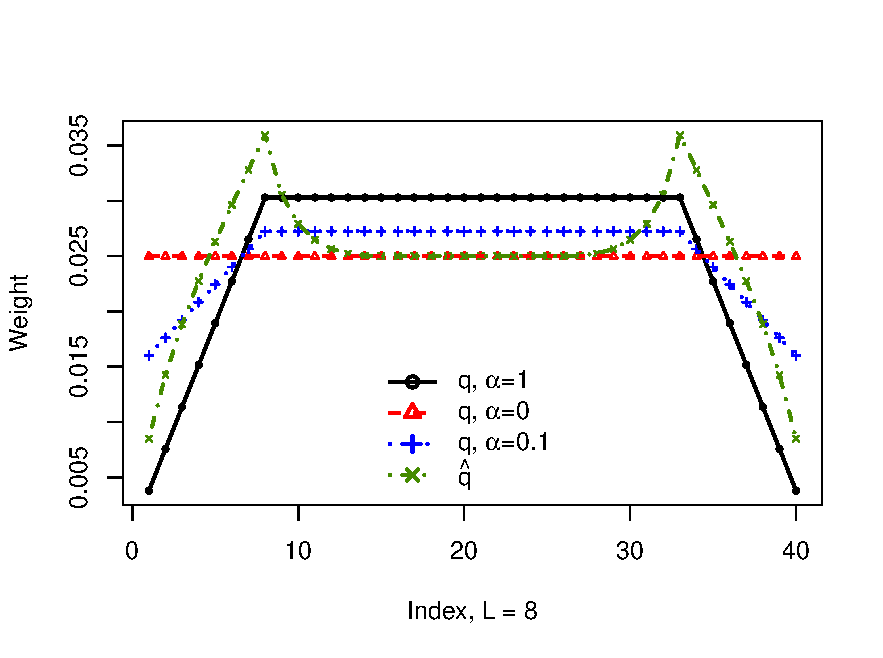
\includegraphics[width = \textwidth]{weights.pdf}\caption{Weights of series elements corresponding to $\bfC(\alpha)$ and $\widehat \bfC$}\label{img_weights}
\end{center}\end{figure}

\subsection{Comments to algorithms. Comparison}

Let us comment and compare the following methods: Weighted Cadzow iterations (Algorithm \ref{alg:WCIt}), Extended Cadzow iterations (Algorithm \ref{alg:ECIt}), Cadzow ($\alpha$) iterations, $0< \alpha \leq 1$, coinciding with usual Cadzow iterations under $\alpha=1$,
and Cadzow $\widehat \bfC$ iterations (Algorithm \ref{alg:obliqueCadzow}).
Note that window length $L$ is a parameter for all considered methods.

\begin{itemize}
\item
The methods are iterative, and convergence to the global minimum in the corresponding Least Squares problem does not necessarily takes place (theoretically, only convergence of subsequences holds; however, there is convergence in the considered examples). %Therefore, comparison of various methods applied to same problem is comprehended.
\item
Theorem \ref{th:converg} provides condition for existence of subsequences convergent to a matrix from $\calM_r \cap \calH$. This theorem is appliable directly to Algorithm \ref{alg:obliqueCadzow} if all weights are positive and to Algorithm \ref{alg:WCIt} if the weighted projection to $\calM_r$ can be calculated with no error. It is easy to extend Theorem \ref{th:converg} to Algorithm \ref{alg:ECIt} where the weights for added values are zero. Note that matrices $\tilde \bfY_k$ consisting of columns of matrices $\Pi_{\calM_r} \bfY_k$ from $L$-th to $N$-th and having positive weight of each element are matrices of rank not larger than $r$, and their Frobenius norms are not larger than seminorm of original matrix: $\|\tilde \bfY_k\|_F \le \|\Pi_{\calM_r} \bfY_k\|_\bfM$, so it is bounded sequence which contains a subsequence converging to needed set.
\item
Accuracy of estimation of extracted signal $\bfS$ is our point of interest, not an error of approximation of the initial series $\tsX$. Generally, it is possible that too accurate approximation of the given series could lead to overfitting, so that the quality of the signal estimation decreases.
\item
Weighted and Extended Cadzow iterations solves problem \eqref{L-rank_task} with equal weights $q_i$. Other methods work with weights with various degree of non-uniformity.
\item
However, each iteration in Weighted and Extended Cadzow algorithms distinguishes by higher computational complexity since it uses one more iterative algorithm on each outer step.
\item
Computational complexity is described by both complexity of one iteration and amount of iterations. Evidently, the number of iterations is determined by convergence rate.
\item
One iteration of Cadzow iterations is well-known Singular Spectrum Analysis (SSA) method, which can solve significally wider range of tasks than the iterative method does. Therefore, precision of signal estimation done by one iteration in all described methods is the point of interest together with the limiting value.
\item
Separability, which defines the ability of a method to (approximately) find a signal using given series, is the one of important concepts of the SSA method. In particular, separability accuracy is closely related to precision of the first iteration of the method. Hence, it is naturally to assume that precision of first iteration is connected with method's convergency rate. Therefore, questions about separability accuracy are related to convergency speed of iterative methods.
\item
The connection between separability and window length $L$ is well researched for the SSA method, see \cite{Golyandina2010}. In particular, an optimal window length is near to half of the series length. Small window length $L$ tends to poor separability. Influence of parameter $\alpha$ in the class of Cadzow ($\alpha$) iterations is researched in Appendix (\ref{sec:app}) on the example of separability of constant and harmonic signal. It is shown that small value of $\alpha$ tends to poor separability, though this case corresponds to approximately equal weights $q_i$ in problem \eqref{L-rank_task}. Generally, the following effect becomes clear: parameters ($\alpha$ as well as $L$) corresponding to more uniform weights lead to worse separability.
\item
It seems that fast convergence speed and high precision of estimation of signal are properties that can not be satisfied simultaneously. Probably this is caused by contradiction between uniformity of weights and separability. Also, it seems that slow convergence can help to find a better solution of the optimization problem.
\end{itemize}

\begin{remark}
\label{rem:adjust}
Adjustment \eqref{eq:adjust} defined in can be applied to $\widehat\tsS$ in all algorithms. In \eqref{eq:adjust} $\|\cdot\|$ is standard Euclidean norm not depending on algorithms, because since this norm corresponds to problem \eqref{L-rank_task} with equal weights $q_i$. We will call the algorithms with adjustment \eqref{eq:adjust} adjusted algorithms. For example, result of the $k$-th iteration of the Cadzow iterations method can be written as $\widehat\tsS_k = \calT^{-1}(\Pi_\calH \Pi_{\calM_r})^k \calT \tsX$. Then the result of the $k$-th iteration of the adjusted Cadzow iterations method is $\widehat\tsS_k^*=\calA(\widehat\tsS_k)$.
\end{remark}

\section{Numeric examples}
\label{sec:simul}
Let us consider numerical experiments for analysis of performance of the considered methods. Comparison of methods was done on examples with a sine wave signal exponentially-modulated sine wave signal.
Since results are very similar, only results for the sine wave signal are presented.

Let the signal $\tsS = (s_{1}, \ldots, s_N)$ of length $N = 40$ have form:
\begin{equation*}
s_{i} = 5\sin{\frac{2 \pi k}{6}}, \quad k = 1, \ldots, N,
\end{equation*}
and the series $\tsX = \tsS + \tsN$ is observed, where  $\tsN$ is Gaussian white noise with mean equal to $0$ and variance equal to $1$. Precision of signal estimation $\widehat\tsS$ is is calculated as root of mean squared error (RMSE) using 1000 repeats Comparison is performed on the same simulated samples. It was checked that comparison results are significant at 5\% level of significance.

We start with investigation of the Cadzow ($\alpha$) methods and the Cadzow with $\widehat \bfC$ method. These methods use oblique SVD; Cadzow($1$) is the conventional Cadzow method. Figure \ref{img_cadzowspeed2} shows the rate of convergence for $\alpha = 0.1$ and $1$ and two different window lengths $L$. There are iteration number on X axis, and RMSE of signal estimate divided by number of measurements in series on Y axis.

\begin{figure}[!hhh]
\begin{center}
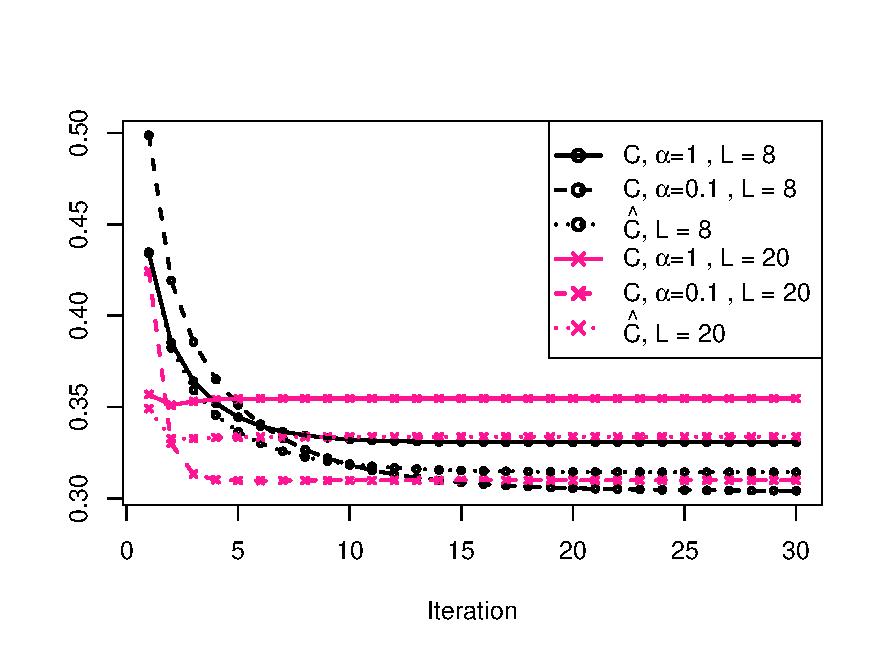
\includegraphics[width = \textwidth]{cadzowspeed_2.pdf}
\caption{RMSE of signal estimate depending on number of iterations.}
\label{img_cadzowspeed2}
\end{center}
\end{figure}

One can see that the method with the smallest limit error is the one with slowest convergence rate. For the considered parameters, it is Cadzow (0.1) with window length $L=8$, where also, weights \emph{corresponding to this method} \footnote{ссылка} are most uniform.
Note that the precision does not differ strongly, from 0.31 ($\alpha=0.1$, $L=8$) in the best case to 0.35 ($\alpha=1$, $L=20$) in the worst case. However, error 0.35 is achieved at first iteration in the first case, while it takes 4--5 iterations to achieve error 0.35 in the second case.

Consider estimation error spreading behavior by series measurements in detail including Extended and Weighted Cadzow iterations. Number of iterations equal to 100 is taken as stop criterion STOP1 (this choice yields the error close to the limiting value), and stop criterion STOP2 for inner iterations is as follows:
 $\frac{\|\bfY_k - \bfY_{k+1}\|^2}{LK} < 10^{-4}$. Initial left and right extended values $\tsL_{L-1}$ и $\tsR_{L-1}$ in Extended Cadzow iterations are obtained using Vector SSA forecast \cite[chapter 2.3.1]{Golyandina.etal2001}.

Figures~\ref{fig:s1_it1}~and~\ref{fig:s1_it100} show the dependence of RMSE for each series point. Picture~\ref{fig:s1_it1} shows errors at first iteration, Picture~\ref{fig:s1_it100} shows errors at 100-th iteration. It is clear that Extended Cadzow method is the most precise in both cases. Cadzow and Cadzow with $\widehat\bfC$ methods are the best at first iteration among methods without inner iterations. The best method in the limit (after 100-th iteration, results do not change significally further) is Cadzow with $\alpha=0.1$, and it is not surprising according to Figure~\ref{img_cadzowspeed2}.

\begin{figure}[!hhh]
\begin{center}
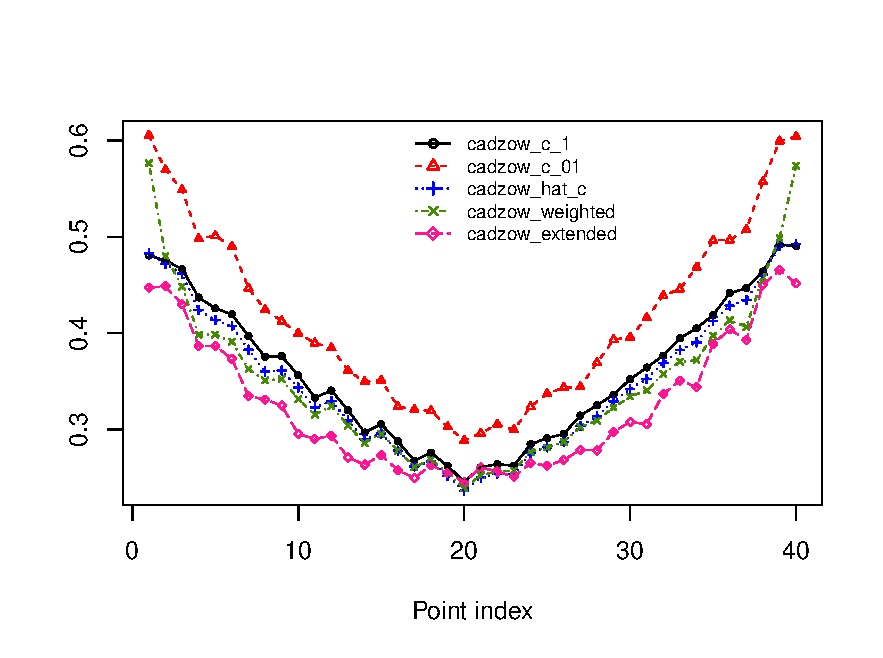
\includegraphics[width = 13cm]{s1_it1.pdf}
\caption{RMSE of signal estimate at each series point; iteration 1.}
\label{fig:s1_it1}
\end{center}
\end{figure}

\begin{figure}[!hhh]
\begin{center}
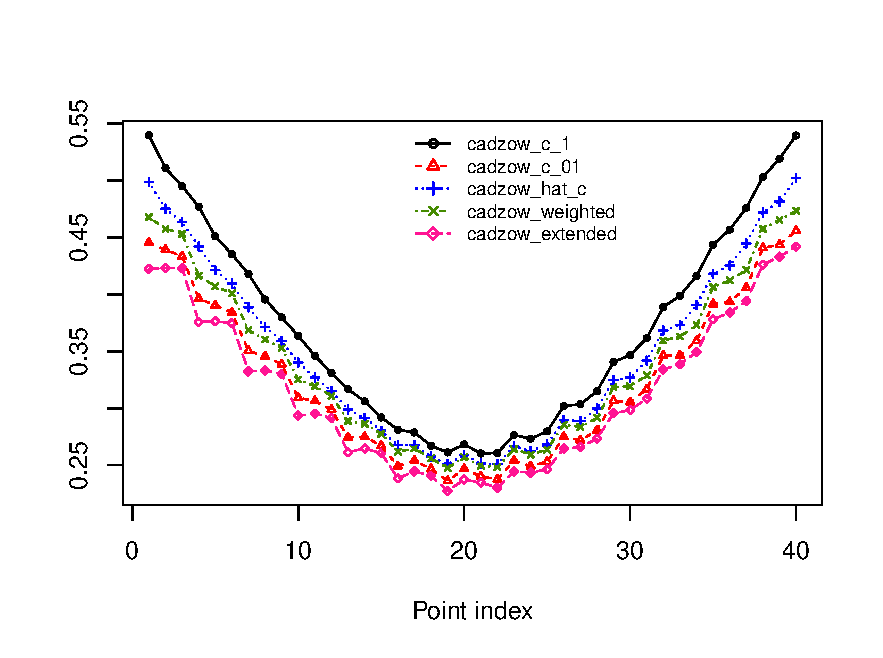
\includegraphics[width = 13cm]{s1_it100.pdf}
\caption{RMSE of signal estimate at each series point; iteration 100.}
\label{fig:s1_it100}
\end{center}
\end{figure}

Consider Table~\ref{fintable} which shows method results, namely, RMSE for $\tilde \tsS$ as an estimate of the signal $\tsS$ and for $\tilde \tsS$ as an estimate of the initial series $\tsX$. \footnote{(that is, as the approximation error) -- не понял} Here $k$ is the number of iterations, $L=20$. Table~\ref{fintable} confirms conclusions about comparison of methods by precision of signal estimation. Also it is seen that еру quality of initial series approximation does not always correspond with quality of signal estimation. For example, overfitting is clearly present for Cadzow ($0.1$) iterations at first iteration. However, methods are ordered identically by precision of approximation and precision of signal estimation in the limit.

The same experiments were performed with adjusted algorithms (see Remark~\ref{rem:adjust}). One can see in Table~\ref{fintable_improved} that the accuracy is almost the same. Adjustment improves approximation of initial series in all cases by its construction, however, the influence to precision of signal approximation is ambiguous (it improves precision at 100th iteration; results are various at first iteration).

\begin{table}[!hhh]
\begin{center}
\caption{Comparison of methods by RMSE, $L = 20$}\label{fintable}
\begin{tabular}{|c|c|c|c|c|}
\hline
$P$: & $\tsS$, $k = 1$ & $\tsX$, $k = 1$ & $\tsS$, $k = 100$ & $\tsX$, $k = 100$  \\
\hline
Cadzow, $\alpha = 1$ & 0.3758 & 0.9195 & 0.3782 & 0.9664 \\
\hline
Cadzow, $\alpha = 0.1$ & 0.4329 & 0.7040 & 0.3311 & 0.9506 \\
\hline
Cadzow $\hat{\bfC}$ & 0.3655 & 0.8925 & 0.3559 & 0.9583 \\
\hline
Weighted Cadzow & 0.3644 & 0.8891 & 0.3455 & 0.9549 \\
\hline
Extended Cadzow & 0.3361 & 0.9030 & 0.3189 & 0.9471 \\
\hline
\end{tabular}
\end{center}
\end{table}

\begin{table}[!hhh]
	\begin{center}
		\caption{Comparison of adjusted methods by RMSE, $L = 20$}\label{fintable_improved}
		\begin{tabular}{|c|c|c|c|c|}
			\hline
			$P$: & $\tsS$, $k = 1$ & $\tsX$, $k = 1$ & $\tsS$, $k = 100$ & $\tsX$, $k = 100$  \\
			\hline
			Cadzow, $\alpha = 1$ & 0.3714 & 0.9175 & 0.3667 & 0.9622 \\
			\hline
			Cadzow, $\alpha = 0.1$ & 0.4385 & 0.7023 & 0.3276 & 0.9493 \\
			\hline
			Cadzow $\hat{\bfC}$ & 0.3626 & 0.8909 & 0.3478 & 0.9555 \\
			\hline
			Weighted Cadzow & 0.3640 & 0.8883 & 0.3380 & 0.9523 \\
			\hline
			Extended Cadzow & 0.3370 & 0.9030 & 0.3184 & 0.9469 \\
			\hline
		\end{tabular}
	\end{center}
\end{table}

\section{Conclusion}
\label{sec:concl}
Several known and new iterative algorithms for approximation of a noisy series by a finite-rank series (signal) were considered in the paper. The approximation was performed by Least Squares method and was considered as an estimate of signal.

\footnote{С этого места --- переписать}Large class of algorithms was reviewed with aim of achieving equal weights in Least Squares method. Equal weights were achieved by using inner iterations only, which converges to local minimum only and makes algorithms time-consuming. Usage of methods without inner iterations leads to approximately equal weights only.

Convergency of outer iterations by subsequences was proved for reviewed class of algorithms.

Results about precision and convergency speed of considered methods were obtained by simulation on the example of noisy sine signal. Results shows that the most precise is the most time-consuming method. Questions about relation of convergency speed, computational complexity and precision of methods were reviewed. Also, emphasis was placed on precision of estimate made by one iteration of methods.

Further work includes extended numeric and analytical research of methods, and achievement of more specific recomendations about relation of computational complexity and precision.

%\bibliographystyle{plain}
\bibliographystyle{gost2008}
\bibliography{zvonarev}
\addcontentsline{toc}{section}{References}

\section{Appendix: separability of constant and harmonic signal for Oblique Cadzow iterations}
\label{sec:app}

Let us introduce another characteristic of algorithms showing ability of decomposing time series into additive parts. Basic application of described algorithms is the problem of signal estimation, so that characteristic is important for obtaining a more precise estimate as much as possible.

Let $\bfC \in \sfR^{K \times K}$ be symmetric semidefinite matrix, $\tsX_1$ и $\tsX_2$ ---  two different time series of length $N$, $\bfX^1$, $\bfX^2$ --- their trajectory matrices. Then define \emph{correlation coefficient of $i$-th and $j$-th column} by:
\begin{equation}\label{col_corr}
\rho^c_{i,j} = \frac{(X^1_i, X^2_j)}{\|X^1_i\| \|X^2_j\|},
\end{equation}
where $X^k_i$ is $i$-th column of matrix $\bfX^k$, $k = 1, 2$, $(\cdot, \cdot)$ is euclidian inner product, $\|\cdot\|$ is euclidean norm. Define \emph{correlation coefficient of $i$-th and $j$-th row} by:
\begin{equation}\label{row_corr}
\rho^r_{i,j} = \frac{(X^{1,i}, X^{2,j})_\bfC}{\|X^{1,i}\|_\bfC \|X^{2,j}\|_\bfC},
\end{equation}
where $X^{k,i}$ is $i$-th row of matrix $\bfX^k$, $k = 1, 2$, and $(\cdot, \cdot)_\bfC$ is oblique inner product generated by matrix $\bfC$ in $\sfR^K$ defined as follows: $(X, Y)_\bfC = X \bfC Y^\sfT$, because $X$ and $Y$ are row-vectors, $\| \cdot \|_\bfC$ is the norm with respect to this inner product. Let us say that series $\tsX_1$ and $\tsX_2$ are \emph{weak $\varepsilon$---separatable} if
\begin{equation}\label{weak_sep_eq}
\rho = \max\Big(\max_{1 \le i,j \le K}|\rho^c_{i,j}|, \max_{1 \le i,j \le L}|\rho^r_{i,j}|\Big) < \varepsilon.
\end{equation}
We are interested in order of $\varepsilon$ for various matrices $\bfC$ and series $\tsX_1 = (c, c, \ldots)$ --- some constant series and $\tsX_2 = (\cos(2 \pi \omega k), k = 1, 2, \ldots)$, and also for various $L$ and $K$ under assumption that only first $N = L + K - 1$ measurements of series are taken. When $\bfC$ is identity matrix, the answer is known: $\varepsilon$ have order $1/\min(L,K)$, i.e. speed of convergency have order $1/N$ for $L$ proportional to $N$.
This result could be found in \cite[Chapter 6.1]{Golyandina.etal2001}. This result relates to the precision of first iteration of Cadzow iterations.

Order of separability of Cadzow ($\alpha$) iterations, introduced in Chapter~\ref{sec:cadzow_alpha}, is considered in following proposition.

\begin{proposition}
\label{prop:separ1}
Let $\tsX_1 = (c, c, \ldots)$ be some constant and $\tsX_2 = (\cos(2 \pi \omega k), k = 1, 2, \ldots)$, where $0<\omega <0.5$, $L,K\ra \infty$ such that $h = h_L = N/L$, where $N=L+K-1$, is integer, and $\bfC$ defined in Cadzow ($\alpha$) iterations, i.e.  $\bfC$ is diagonal matrix with following diagonal elements:
\begin{equation*}
c_k = \begin{cases}
1, & \text{если} \quad k = jL+1 \quad \text{for some} \ j = 0, \ldots, h-1,\\
\alpha, & \text{otherwise},
\end{cases}
\end{equation*}
where $0 \le \alpha \le 1$. Then $\rho$ have order $\max(\frac{1}{L}, \frac{(1-\alpha)C_{L,K}+\alpha}{(1-\alpha)N/L+\alpha K})$, where order of $C_{L,K}$
could vary from $O(1)$ to $O(N/L)$ depending on how $K$ tends to infinity.
\end{proposition}

\begin{proof5}{\ref{prop:separ1}}
It is necessary to evaluate an order of following values:
\begin{gather*}
\rho^c_{i,j} = \frac{\sum_{k=j}^{j + L - 1} \cos(2 \pi \omega k)}{\sqrt{L (\sum_{k=j}^{j + L - 1} \cos^2(2 \pi \omega k))}},\\ \rho^r_{i,j} = \frac{\sum_{k=1}^K c_k\cos(2 \pi \omega (j + k - 1))}{\sqrt{(\sum_{k=1}^K c_k) (\sum_{k=1}^K c_k\cos^2(2 \pi \omega (j + k - 1)))}}.
\end{gather*}
Let us use following facts to prove the proposition:
\begin{gather*}
\sum_{k=1}^n \cos(ak + b) = \csc(a/2) \sin(an / 2) \cos \left(\frac{an + a + 2b}{2} \right), \\
\sum_{k=1}^n \cos^2(ak + b) = \frac{1}{4}(\csc(a) \sin(2an + a + 2b) -\\ - \csc(a)\sin(a + 2b) + 2n),
\end{gather*}
for any real $a, b$ and positive integer $n$.
Thus when series $\tsX_2$ is not constant, numerator in $\rho^c_{i,j}$ have order $O(1)$, and denominator --- $O(L)$.
First part is proved, and its proof is exactly analogous to the case when $\bfC$ is identity matrix.

To prove second part choose a sum for $k$ such that $c_k=1$ separately:
\begin{gather*}
\sum_{k=1}^K c_k\cos(2 \pi \omega (j + k - 1)) = (1-\alpha) \sum_{\substack{1 \le k \le K: \\ c_k = 1}}\cos(2 \pi \omega (j + k - 1)) +\\ +\sum_{1 \le k \le K}\alpha \cos(2 \pi \omega (j + k - 1)) = (1-\alpha) C_{L,K} + \alpha\, O(1),
\\
%\end{gather*}
%\begin{gather*}
\sum_{k=1}^K c_k = (1-\alpha) N/L + \alpha K,
\\
%\end{gather*}
%\begin{gather*}
\sum_{k=1}^K c_k\cos^2(2 \pi \omega (j + k - 1)) = (1-\alpha)\sum_{\substack{1 \le k \le K: \\ c_k = 1}}\cos^2(2 \pi \omega (j + k - 1)) +\\ +\sum_{1 \le k \le K }\alpha \cos^2(2 \pi \omega (j + k - 1)) = (1-\alpha) O(N/L) + \alpha\, O(K).
\end{gather*}
In the worst case when $L\omega$ is integer we obtain that $\cos(2 \pi \omega (j + k - 1))$ is a constant not depending from $j$ and $k$, and then $C_{L,K}$ has order $O(N/L)$.
\end{proof5}

Thus even in the worst case when $C_{L,K}$ has order $O(1)$, separability of constant and sine signal becomes worse than in usual Cadzow iterations: for $\alpha$ close to 0, the most optimal chose for $L$ is $L \approx \sqrt{N}$, so order of separability equal to $1/\sqrt{N}$ is obtained.

Now let us consider Cadzow with $\widehat\bfC$ iterations introduced in Chapter~\ref{sec:cadzow_hat}.

\begin{proposition}
\label{prop:separ2}
Let $\tsX_1 = (c, c, \ldots)$ be some constant signal and $\tsX_2 = (\cos(2 \pi \omega k), k = 1, 2, \ldots)$, where $0<\omega <0.5$, $L,K\ra \infty$ and $\bfC$ defined in Cadzow with $\widehat\bfC$ iterations.
 Then $\rho$ have order $\max \left(1/L, \frac{H_L}{\sqrt{NK}} \right)$ as $L, K \to \infty$, where $H_L$ is $L$-th harmonic number.
\end{proposition}

\begin{proof5}{\ref{prop:separ2}}
It is necessary to evaluate an order of following values:
\begin{gather*}
\rho^c_{i,j} = \frac{\sum_{k=j}^{j + L - 1} \cos(2 \pi \omega k)}{\sqrt{L (\sum_{k=j}^{j + L - 1} \cos^2(2 \pi \omega k))}}, \\ \rho^r_{i,j} = \frac{\sum_{k=1}^K \hat c_k\cos(2 \pi \omega (j + k - 1))}{\sqrt{(\sum_{k=1}^K \hat c_k) (\sum_{k=1}^K \hat c_k\cos^2(2 \pi \omega (j + k - 1)))}}.
\end{gather*}
 The order of $\rho^c_{i,j}$ was already obtained in proof of Proposition~\ref{prop:separ1}, so let us just move to $\rho^r_{i,j}$. Consider the correlation of first rows only --- proof for remained rows is absolutely analogous. Consider a numerator $\rho^r_{1,1}$:
\begin{gather*}
\sum_{k=1}^K \hat c_k\cos(2 \pi \omega k) = \sum_{k=1}^{L-1} \hat c_k\cos(2 \pi \omega k) + \sum_{k=L}^{K - L + 1} \frac{\cos(2 \pi \omega k)}{L} +\\+ \sum_{k=K - L + 2}^{K} \hat c_k\cos(2 \pi \omega k) = I_1 + I_2 + I_3,
\end{gather*}
which is divided by three parts. For $I_2$ an estimate $O(1/L)$ is carried out, and the proof for $I_3$ is analogic to proof for $I_1$:
\begin{gather*}
|I_1|=\bigg|\sum_{k=1}^{L-1}\frac{1}{L}\left(\frac{k}{L} + \sum_{j=k}^{L-1} \frac{1}{j} \right) \cos(2 \pi \omega k)\bigg| =\\= \bigg|\sum_{k=1}^{L-1} \frac{k \cos(2 \pi \omega k)}{L^2} +  \frac{1}{L}\sum_{k = 1}^{L-1}\sum_{j = k}^{L-1}\frac{\cos(2 \pi \omega k)}{j}\bigg| \le \\ \le
\bigg|\sum_{k=1}^{L-1} \frac{k \cos(2 \pi \omega k)}{L^2}\bigg| + \bigg|\frac{1}{L}\sum_{k = 1}^{L-1}\sum_{j = k}^{L-1}\frac{\cos(2 \pi \omega k)}{j}\bigg|.
\end{gather*}
Using a fact that
\begin{gather*}
\sum_{k=1}^n k \cos(ak + b) = -\frac{1}{4}\csc^2(a/2)(-(n+1)\cos(an+b) + \\ + n\cos(an + a + b) + \cos b),
\end{gather*}
obtain that:
\begin{gather*}
\bigg|\sum_{k=1}^{L-1} \frac{k \cos(2 \pi \omega k)}{L^2}\bigg| = O(1/L), \quad
\bigg|\frac{1}{L}\sum_{k = 1}^{L-1}\sum_{j = k}^{L-1}\frac{\cos(2 \pi \omega k)}{j}\bigg| = \\ =\bigg|\frac{1}{L}\sum_{j = 1}^{L-1}\sum_{k = 1}^{j}\frac{\cos(2 \pi \omega k)}{j}\bigg| \le \bigg|\frac{1}{L}\sum_{j = 1}^{L-1}\frac{d}{j}\bigg| = O \left(\frac{H_L}{L} \right),
\end{gather*}
where $d$ is some constant.

Following sums are considered for the denominator:
\begin{equation*}
\sum_{k=1}^K \hat c_k = N / L
\end{equation*}
by definition, and the following part is just estimated lower:
\begin{equation*}
\sum_{k=1}^K \hat c_k\cos^2(2 \pi \omega (j + k - 1)) \ge \sum_{k=1}^K \frac{1}{L}\cos^2(2 \pi \omega (j + k - 1)) = O \left(\frac{K}{L} \right).
\end{equation*}
\end{proof5}


\end{document}
